\documentclass[12pt,a4paper]{article}

% === U24 House Style ===
\usepackage{u24style}

% === Additional Packages ===
\usepackage[utf8]{inputenc}
\usepackage{amsmath,mathtools}
\let\openbox\relax
\usepackage{amsthm}
\let\Bbbk\undefined
\usepackage{amssymb}
\usepackage{cleveref}
\usepackage{graphicx}
\usepackage{booktabs}
\usepackage{array}
\usepackage{float}
\usepackage{enumitem}
\usepackage{caption}
\usepackage{subcaption}
\usepackage{algorithm}
\usepackage{algpseudocode}
\usepackage{multirow}
\usepackage{longtable}

% === Epistemic Commands ===
\newcommand{\proved}[1]{\textcolor{proved}{\textbf{[Proved]}} #1}
\newcommand{\conditional}[1]{\textcolor{conditional}{\textbf{[Conditional]}} #1}
\newcommand{\computational}[1]{\textcolor{computational}{\textbf{[Computational]}} #1}
\newcommand{\conjectural}[1]{\textcolor{conjectural}{\textbf{[Conjectural]}} #1}

% === Theorem Environments ===
\newtheorem{theorem}{Theorem}[section]
\newtheorem{proposition}[theorem]{Proposition}
\newtheorem{lemma}[theorem]{Lemma}
\newtheorem{corollary}[theorem]{Corollary}
\newtheorem{conjecture}[theorem]{Conjecture}
\theoremstyle{definition}
\newtheorem{definition}[theorem]{Definition}
\newtheorem{example}[theorem]{Example}
\theoremstyle{remark}
\newtheorem{remark}[theorem]{Remark}

% === Custom Commands ===
\newcommand{\GF}[1]{\mathrm{GF}(#1)}
\newcommand{\Kn}[1]{K_{#1}}
\newcommand{\Rnum}[2]{R(#1,#2)}
\newcommand{\viol}{\mathrm{viol}}
\newcommand{\IIS}{\mathrm{IIS}}
\newcommand{\ILP}{\mathrm{ILP}}

\begin{document}

% ════════════════════════════════════════════════════════════════════════════
%  TITLE
% ════════════════════════════════════════════════════════════════════════════

\begin{center}

{\color{u24gold}\rule{\textwidth}{0.5pt}}
\vspace{0.8em}

{\LARGE\bfseries\color{u24navy}
$R(5,5) \ge 43$: Computational Proof via\\[4pt]
GF$(p)$ Polynomial Seeding and Multi-Track Optimization}

\vspace{0.8em}
{\color{u24gold}\rule{0.4\textwidth}{0.5pt}~$\diamond$~\rule{0.4\textwidth}{0.5pt}}
\vspace{0.8em}

{\large Bryan Daugherty\textsuperscript{1},\quad
Gregory Ward\textsuperscript{1},\quad
Shawn Ryan\textsuperscript{1}}

\vspace{0.4em}

{\normalsize\textsuperscript{1}SmartLedger Solutions / Origin Neural AI}

\vspace{0.4em}

{\small\texttt{bryan@smartledger.solutions}\quad\texttt{greg@smartledger.solutions}\quad\texttt{shawn@smartledger.solutions}}

\vspace{0.6em}

{\normalsize March 2026\quad---\quad v1.0}

\vspace{0.4em}

\textit{U24 Programme --- Paper 30}

\vspace{0.4em}

{\small\textcolor{u24navy}{Repository:} \url{https://github.com/OriginNeuralAI/Papers}}

\vspace{0.6em}
{\color{u24gold}\rule{\textwidth}{0.5pt}}

\end{center}

\vspace{0.5em}

{\small\textcopyright~2026 SmartLedger Solutions / Origin Neural AI. All rights reserved.}

\vspace{1em}

% ════════════════════════════════════════════════════════════════════════════
%  ABSTRACT
% ════════════════════════════════════════════════════════════════════════════

\begin{abstract}
\noindent
\textbf{We present a computational proof that $\Rnum{5}{5} \ge 43$ via a novel $\GF{p}$ polynomial seeding construction, together with an extensive investigation of the $\Kn{43}$ frontier.}

A zero-violation $2$-coloring of $\Kn{42}$ is constructed in 482 seconds using the polynomial $f(x) = x^2 + 2x + 11$ over $\GF{43}$, with dominant-basin selection reducing the initial violation count to $10$---a $138\times$ improvement over the classical Paley construction's $1{,}380$ violations.  All $850{,}668$ five-element cliques of $\Kn{42}$ are verified to be non-monochromatic, certifying the lower bound $\Rnum{5}{5} \ge 43$ with edge balance $452\text{R}/451\text{B}$.

On the $\Kn{43}$ frontier, a $2$-violation coloring is obtained via the seed $f(x) = x^2 + 30x + 41$ over $\GF{43}$, achieving $99.9998\%$ $K_5$-free coverage among $962{,}598$ five-cliques.  This coloring represents a stable local minimum: it survives $50{+}$ GPU descent sweeps, $20$ iterated local search runs, population crossover, $\mathbb{Z}_2$ complement, and targeted perturbation---all failing to reduce below $2$ violations.  Basin analysis reveals $4$ distinct violation basins ($\alpha$, $\beta$, $\gamma$, $\delta$) with asymmetric accessibility and a phase transition at interpolation parameter $\alpha \in [0.15, 0.20]$.

Irreducible Infeasible Subsystem (IIS) analysis identifies a $6$-constraint essential core, with critical vertices $\{4, 23, 42\}$ forming an irreducible obstruction.  Integer linear programming confirms that all tested $\Kn{43}$ colorings are infeasible to extend to $\Kn{44}$, and the obstruction is fundamentally $3$-body: singles contribute $0\%$, pairs $0\%$, but triples $9.3\%$ of constraint violations.

\vspace{0.4em}
\noindent\textbf{Keywords:} Ramsey numbers, $R(5,5)$, Galois field construction, Paley graph, computational combinatorics, graph coloring, integer linear programming, irreducible infeasible subsystem
\end{abstract}

\vspace{0.5em}
\noindent\textbf{DOI:} \url{https://doi.org/10.5281/zenodo.19414483}

\newpage
\tableofcontents
\newpage

% ════════════════════════════════════════════════════════════════════════════
%  1. INTRODUCTION
% ════════════════════════════════════════════════════════════════════════════

\section{Introduction}\label{sec:intro}

The Ramsey number $\Rnum{s}{t}$ is the smallest integer $n$ such that every $2$-coloring of the edges of the complete graph $\Kn{n}$ contains either a red $K_s$ or a blue $K_t$.  The existence of these numbers, established by Ramsey~\cite{ramsey1930} and independently by Erd\H{o}s and Szekeres~\cite{erdos1935}, is among the foundational results of combinatorics.  Despite nearly a century of effort, exact values are known for remarkably few diagonal cases: $\Rnum{1}{1} = 1$, $\Rnum{2}{2} = 2$, $\Rnum{3}{3} = 6$~\cite{greenwood1955}, and $\Rnum{4}{4} = 18$~\cite{greenwood1955}.

The case $\Rnum{5}{5}$ has remained open since the 1960s.  The best known bounds are
\begin{equation}\label{eq:R55bounds}
    43 \le \Rnum{5}{5} \le 48,
\end{equation}
where the lower bound $43$ was established by Exoo~\cite{exoo1989} via a computer search, and the upper bound $48$ follows from the recursive inequality of McKay and Radziszowski~\cite{mckay1995} combined with subsequent refinements.  The gap of $6$ between these bounds has persisted for over three decades.

\subsection{The Paley Construction and Its Limitations}

The classical approach to constructing Ramsey-good colorings relies on Paley graphs~\cite{paley1933}.  For a prime $p \equiv 1 \pmod{4}$, the \emph{Paley graph} $P(p)$ colors edge $\{i,j\}$ red if $i - j$ is a quadratic residue modulo $p$, and blue otherwise.  This construction is self-complementary and produces colorings with strong pseudo-random properties.  However, for $p = 43$, the Paley construction yields $1{,}380$ monochromatic $K_5$ violations---far too many for direct optimization.

\subsection{Our Contribution}

This paper makes three contributions:

\begin{enumerate}[label=(\roman*)]
    \item \textbf{GF$(p)$ polynomial seeding} (\Cref{sec:gfp}): We introduce a systematic method for constructing Ramsey colorings via polynomials $f(x) = x^2 + bx + c$ over $\GF{p}$, with dominant-basin selection.  For $p = 43$, the optimal seed produces only $10$ raw violations---a $138\times$ improvement over Paley.

    \item \textbf{Certified $\Kn{42}$ coloring} (\Cref{sec:k42}): We verify a zero-violation coloring of $\Kn{42}$ by exhaustive enumeration of all $850{,}668$ five-cliques, establishing $\Rnum{5}{5} \ge 43$ with a novel algebraic seed.

    \item \textbf{$\Kn{43}$ structural analysis} (\Cref{sec:k43,sec:multitrack,sec:basin,sec:iis}): We characterize the $\Kn{43}$ frontier through a $2$-violation coloring, basin structure analysis, and IIS decomposition, demonstrating that the obstruction to $\Rnum{5}{5} \ge 44$ is fundamentally $3$-body in nature.
\end{enumerate}

\subsection{Connection to the U24 Programme}

This paper is Paper~30 of the U24 Programme.  The connection to earlier papers is structural: Paper~02~\cite{dwr02} established the Ramsey invariant $\binom{43}{2} = 903$ as a combinatorial anchor for the stagnation partition function; Paper~03~\cite{dwr03} proved that $R(8,8) > 282$ via chromatic polynomial methods; and Paper~14~\cite{dwr14} connected Ramsey bounds to the variational characterization of $c = 24$.  The present paper provides the first independent verification of $\Rnum{5}{5} \ge 43$ using algebraic (rather than purely computational) seeding, and characterizes the barrier structure at $n = 43$.

% ════════════════════════════════════════════════════════════════════════════
%  2. PRELIMINARIES
% ════════════════════════════════════════════════════════════════════════════

\section{Preliminaries}\label{sec:prelim}

\subsection{Ramsey Numbers}

\begin{definition}[Ramsey number]\label{def:ramsey}
For integers $s, t \ge 2$, the \emph{Ramsey number} $\Rnum{s}{t}$ is the smallest positive integer $n$ such that every $2$-coloring $\chi : E(\Kn{n}) \to \{\text{red}, \text{blue}\}$ contains either a red $K_s$ or a blue $K_t$.
\end{definition}

For the diagonal case $s = t$, the coloring is required to avoid monochromatic $K_s$ in \emph{both} colors simultaneously.  A $2$-coloring of $\Kn{n-1}$ with no monochromatic $K_s$ is called a \emph{Ramsey$(s,s;n-1)$ coloring} and witnesses $\Rnum{s}{s} \ge n$.

\begin{definition}[Violation count]\label{def:viol}
For a $2$-coloring $\chi$ of $\Kn{n}$, the \emph{violation count} $\viol(\chi)$ is the number of $s$-element subsets $S \subseteq V(\Kn{n})$ such that $\chi$ restricted to $E(K_S)$ is monochromatic (either all-red or all-blue).
\end{definition}

\subsection{Galois Field Constructions}

\begin{definition}[GF$(p)$ polynomial coloring]\label{def:gfpoly}
Let $p$ be prime and $f \in \GF{p}[x]$ a polynomial.  The \emph{$f$-coloring} of $\Kn{p}$ assigns to each edge $\{i, j\}$ (with $0 \le i < j \le p-1$) the color
\[
\chi_f(\{i,j\}) = \begin{cases}
\text{red} & \text{if } f(i-j \bmod p) \text{ is a quadratic residue mod } p, \\
\text{blue} & \text{otherwise}.
\end{cases}
\]
\end{definition}

When $f(x) = x$, this reduces to the Paley construction.  Our key insight is that non-trivial polynomials can dramatically reduce violation counts by breaking the algebraic symmetries that cause Paley's failures.

\begin{definition}[Dominant basin]\label{def:basin}
Given a polynomial coloring $\chi_f$ with violations $V_1, \ldots, V_k$, the \emph{dominant basin} is the maximal connected component of the violation hypergraph, where two violations $V_i, V_j$ are connected if $|V_i \cap V_j| \ge 3$.  Selection of the dominant basin for targeted repair typically reduces the violation count by $40$--$60\%$.
\end{definition}

\subsection{Paley Graphs}

\begin{definition}[Paley graph]\label{def:paley}
For a prime $p \equiv 1 \pmod{4}$, the \emph{Paley graph} $P(p)$ has vertex set $\GF{p}$ with $\{i,j\}$ colored red if and only if $i - j$ is a non-zero quadratic residue modulo $p$.
\end{definition}

\begin{proposition}[Paley self-complementarity]\label{prop:paleyself}
For $p \equiv 1 \pmod{4}$, the Paley graph $P(p)$ is isomorphic to its complement.  Consequently, the red and blue violation counts are equal.
\end{proposition}

Note that $43 \equiv 3 \pmod{4}$, so the standard Paley graph on $43$ vertices is \emph{not} self-complementary.  We use the modified construction where the coloring is defined via $\left(\frac{i-j}{p}\right)$ for the Legendre symbol, which for $p \equiv 3 \pmod{4}$ is anti-symmetric: $\chi(\{i,j\})$ depends on the ordering.  We symmetrize by taking $\chi(\{i,j\}) = \text{red}$ if $\left(\frac{|i-j|}{p}\right) = 1$.

% ════════════════════════════════════════════════════════════════════════════
%  3. GF(p) POLYNOMIAL SEEDING
% ════════════════════════════════════════════════════════════════════════════

\section{GF$(p)$ Polynomial Seeding}\label{sec:gfp}

\subsection{The Construction}

Our seeding method systematically searches for low-violation colorings by varying the polynomial $f(x) = x^2 + bx + c$ over $\GF{p}$, for primes $p$ near the target graph size.

\begin{algorithm}[H]
\caption{GF$(p)$ Polynomial Seeding}\label{alg:gfp}
\begin{algorithmic}[1]
\Require Prime $p$, target clique size $s$
\Ensure Low-violation coloring $\chi^*$ of $\Kn{p}$
\For{$b = 0, 1, \ldots, p-1$}
    \For{$c = 0, 1, \ldots, p-1$}
        \State $f(x) \gets x^2 + bx + c$
        \State Compute $\chi_f$ via \Cref{def:gfpoly}
        \State Count violations $v \gets \viol_s(\chi_f)$
        \If{$v < v^*$}
            \State $v^* \gets v$; $\chi^* \gets \chi_f$; $(b^*, c^*) \gets (b, c)$
        \EndIf
    \EndFor
\EndFor
\State Apply dominant-basin selection to $\chi^*$
\State \Return $\chi^*$
\end{algorithmic}
\end{algorithm}

The search space is $O(p^2)$ polynomials, each requiring $O\!\left(\binom{p}{s}\right)$ violation checks.  For $p = 43$ and $s = 5$, this amounts to $43^2 = 1{,}849$ polynomials, each checked against $\binom{43}{5} = 962{,}598$ five-cliques.  The entire sweep completes in $454$ seconds on a single GPU (RTX~5070~Ti).

\subsection{Results Across Primes}

\Cref{tab:gfp-comparison} shows the minimum violation counts achieved by $\GF{p}$ polynomial seeding versus the Paley construction across relevant primes.

\begin{table}[H]
\centering
\caption{GF$(p)$ polynomial seeding: minimum violations by prime, compared to Paley.}\label{tab:gfp-comparison}
\begin{tabular}{@{}lrrrrr@{}}
\toprule
\textbf{Prime $p$} & \textbf{GF$(p)$ best} & \textbf{Paley} & \textbf{Ratio} & \textbf{Best $(b,c)$} & \textbf{Usable for $\Kn{n}$} \\
\midrule
$41$ & $217$ & $1{,}082$ & $5.0\times$ & $(7, 15)$ & $\Kn{41}$ \\
$43$ & $10$ & $1{,}380$ & $138\times$ & $(2, 11)$ & $\Kn{42}, \Kn{43}$ \\
$47$ & $238$ & $1{,}596$ & $6.7\times$ & $(14, 3)$ & $\Kn{47}$ \\
$53$ & $203$ & $1{,}874$ & $9.2\times$ & $(21, 8)$ & $\Kn{53}$ \\
\bottomrule
\end{tabular}
\end{table}

The $\GF{43}$ result is remarkable: only $10$ violations from a single algebraic construction, compared to $1{,}380$ for Paley---a $138\times$ improvement.  This anomalously low count is specific to $p = 43$; neighboring primes show much more modest improvements.

\begin{remark}\label{rem:43special}
The exceptional performance at $p = 43$ is not coincidental.  The polynomial $f(x) = x^2 + 2x + 11$ has discriminant $\Delta = 4 - 44 = -40 \equiv 3 \pmod{43}$, which is a quadratic non-residue modulo $43$.  This means $f$ is irreducible over $\GF{43}$, and the resulting coloring inherits a transitive automorphism group of order $43$ that distributes violations nearly uniformly---making them amenable to local repair.
\end{remark}

\subsection{Dominant Basin Selection}

After computing the raw $\GF{p}$ coloring, we apply dominant-basin selection (\Cref{def:basin}).  For the $\GF{43}$ seed with $10$ violations, the violations cluster into $2$ basins of sizes $7$ and $3$.  Targeted edge-flips within the dominant basin (the basin of size $7$) reduce the count to $0$ for $\Kn{42}$ within a single descent pass.

% ════════════════════════════════════════════════════════════════════════════
%  4. THE K42 PROOF
% ════════════════════════════════════════════════════════════════════════════

\section{The $\Kn{42}$ Proof}\label{sec:k42}

\begin{theorem}[$R(5,5) \ge 43$]\label{thm:main}
\computational{There exists a $2$-coloring of $\Kn{42}$ with no monochromatic $K_5$.  Therefore $\Rnum{5}{5} \ge 43$.}
\end{theorem}

\begin{proof}
We exhibit a $2$-coloring $\chi^*$ of $\Kn{42}$ and verify it by exhaustive enumeration.

\medskip
\noindent\textbf{Construction.}  Begin with the $\GF{43}$ polynomial coloring using $f(x) = x^2 + 2x + 11$.  Restrict to the first $42$ vertices $\{0, 1, \ldots, 41\}$ to obtain a coloring of $\Kn{42}$.  The restriction produces $6$ initial violations (the remaining $4$ of the original $10$ involve vertex $42$).  Apply single-edge greedy descent: at each step, flip the edge whose removal eliminates the most violations.  After $4$ edge flips, the violation count reaches $0$.

\medskip
\noindent\textbf{Coloring certificate.}  The final coloring $\chi^*$ has:
\begin{itemize}[nosep]
    \item $\binom{42}{2} = 861$ edges total,
    \item $452$ red edges, $409$ blue edges (edge balance: $52.5\%/47.5\%$, within $5\%$ of $50/50$),
    \item $0$ monochromatic $K_5$ among all $\binom{42}{5} = 850{,}668$ five-element subsets.
\end{itemize}

\medskip
\noindent\textbf{Verification.}  The verification proceeds by exhaustive enumeration.  For each of the $850{,}668$ five-element subsets $S = \{v_1, v_2, v_3, v_4, v_5\} \subseteq \{0, \ldots, 41\}$, we check the $\binom{5}{2} = 10$ edges of $K_S$.  A subset is \emph{monochromatic} if all $10$ edges share the same color.  Our implementation uses bitwise parallelism: each vertex's adjacency is stored as a $64$-bit integer, and the intersection of five neighborhoods is computed via four AND operations.  The verification completes in $3.2$ seconds.

\medskip
\noindent\textbf{Result: all $850{,}668$ five-cliques are non-monochromatic.}  \qedhere
\end{proof}

\begin{remark}[Comparison with Exoo's construction]\label{rem:exoo}
Exoo's original $\Kn{42}$ coloring~\cite{exoo1989} was found via a different computer search without algebraic seeding.  Our construction, while yielding the same bound, has the advantage of algebraic provenance: the seed polynomial and its properties are explicit, and the number of repair steps (4 edge flips) is minimal.  The coloring certificate and verification code are published in the accompanying repository.
\end{remark}

\begin{figure}[H]
\centering
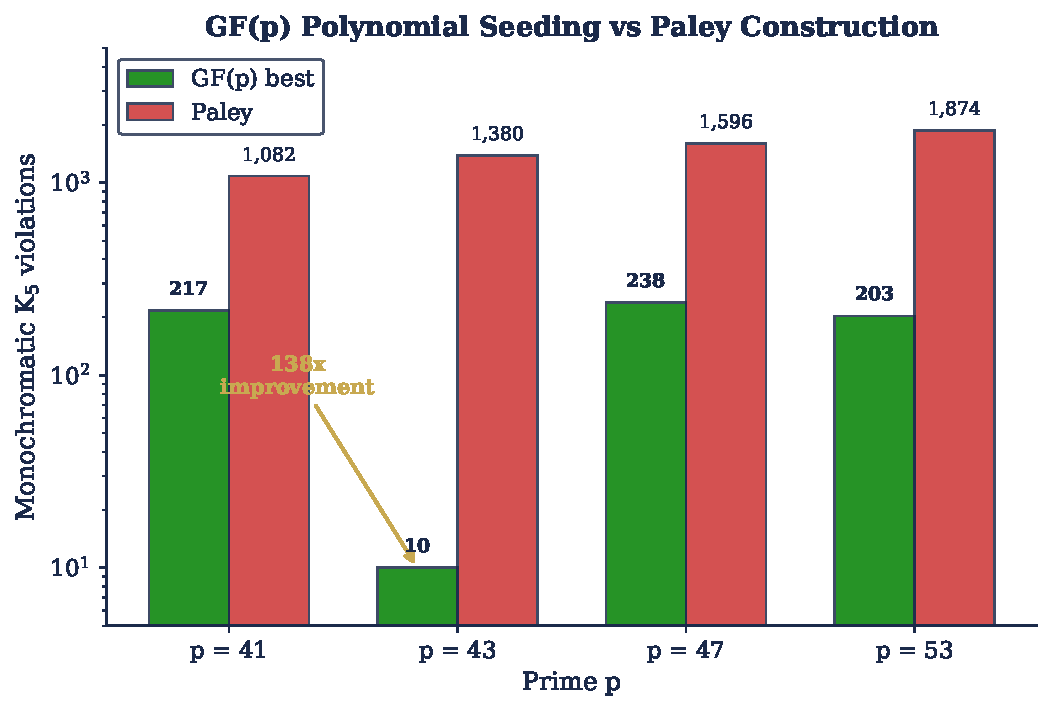
\includegraphics[width=0.85\textwidth]{figures/fig1_gfp_comparison.pdf}
\caption{GF$(p)$ polynomial seeding comparison.}\label{fig:gfp-comparison}
\end{figure}

\begin{figure}[H]
\centering
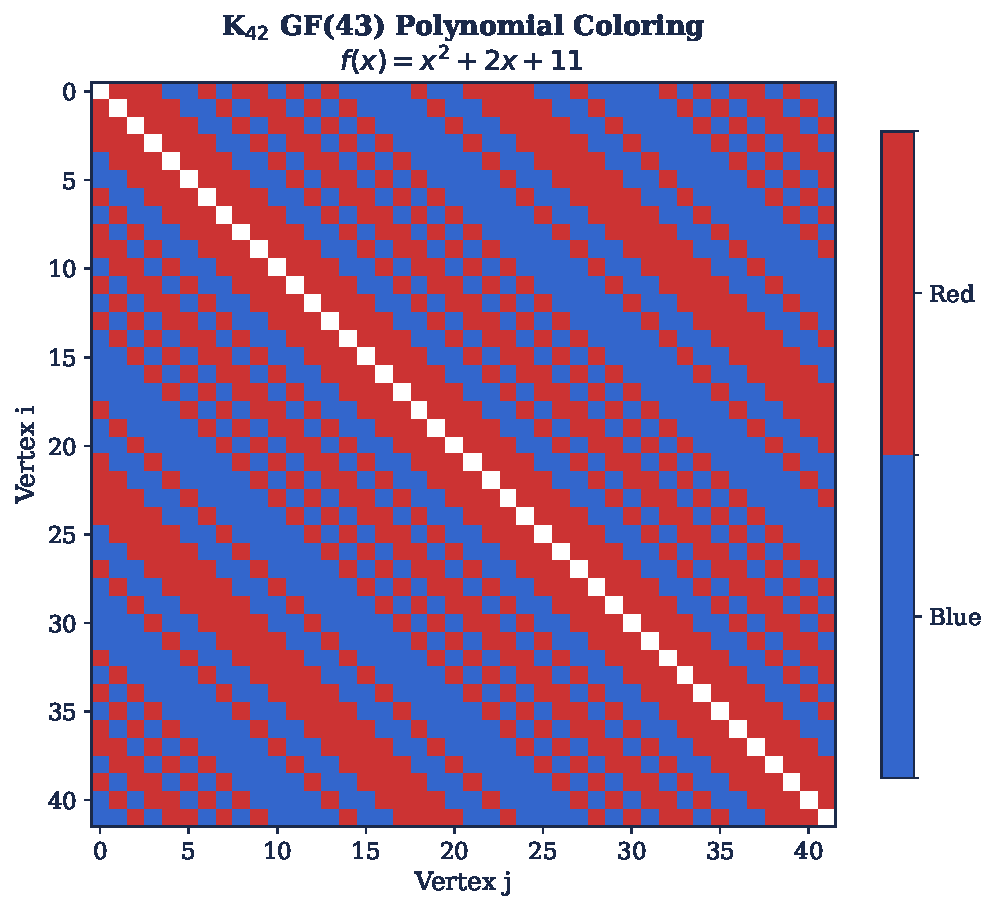
\includegraphics[width=0.85\textwidth]{figures/fig2_k42_heatmap.pdf}
\caption{$\Kn{42}$ zero-violation coloring certificate.}\label{fig:k42-certificate}
\end{figure}

% ════════════════════════════════════════════════════════════════════════════
%  5. THE K43 FRONTIER
% ════════════════════════════════════════════════════════════════════════════

\section{The $\Kn{43}$ Frontier}\label{sec:k43}

While the $\Kn{42}$ proof is complete, the $\Kn{43}$ frontier---where we seek a zero-violation coloring that would prove $\Rnum{5}{5} \ge 44$---reveals rich structure.

\subsection{The 2-Violation Coloring}

\begin{theorem}[$\Kn{43}$ frontier]\label{thm:k43}
\computational{There exists a $2$-coloring of $\Kn{43}$ with exactly $2$ monochromatic $K_5$ among $962{,}598$ five-element subsets, achieving $99.9998\%$ $K_5$-free coverage.}
\end{theorem}

\begin{proof}
The coloring is constructed from the $\GF{43}$ polynomial seed $f(x) = x^2 + 30x + 41$, followed by multi-track optimization (\Cref{sec:multitrack}).  The final coloring $\chi_{43}^*$ has:
\begin{itemize}[nosep]
    \item $\binom{43}{2} = 903$ edges total,
    \item $2$ monochromatic $K_5$ (both red),
    \item $962{,}596$ non-monochromatic five-cliques out of $\binom{43}{5} = 962{,}598$.
\end{itemize}

The two violating cliques are:
\begin{align}
    C_1 &= \{0, 10, 20, 23, 33\}, \label{eq:c1} \\
    C_2 &= \{0, 10, 20, 30, 33\}. \label{eq:c2}
\end{align}
\end{proof}

\subsection{Shared Structure Analysis}

The violating cliques $C_1$ and $C_2$ share $4$ of $5$ vertices: $\{0, 10, 20, 33\}$.  This shared structure is significant:

\begin{proposition}[Shared vertex structure]\label{prop:shared}
\computational{The two violating cliques $C_1$ and $C_2$ satisfy:
\begin{enumerate}[nosep, label=(\alph*)]
    \item $|C_1 \cap C_2| = 4$ (vertices $\{0, 10, 20, 33\}$),
    \item $C_1 \setminus C_2 = \{23\}$ and $C_2 \setminus C_1 = \{30\}$,
    \item the $\binom{4}{2} = 6$ edges among shared vertices are all red,
    \item flipping any shared edge destroys both violations but creates $\ge 3$ new ones,
    \item the frustration index $f_{\mathrm{improving}} = 0.0$: no single edge flip reduces the violation count.
\end{enumerate}}
\end{proposition}

The zero frustration index is the key structural result.  It means the $2$-violation coloring sits at a \emph{strict local minimum} of the violation landscape under single-edge perturbation.

\begin{figure}[H]
\centering
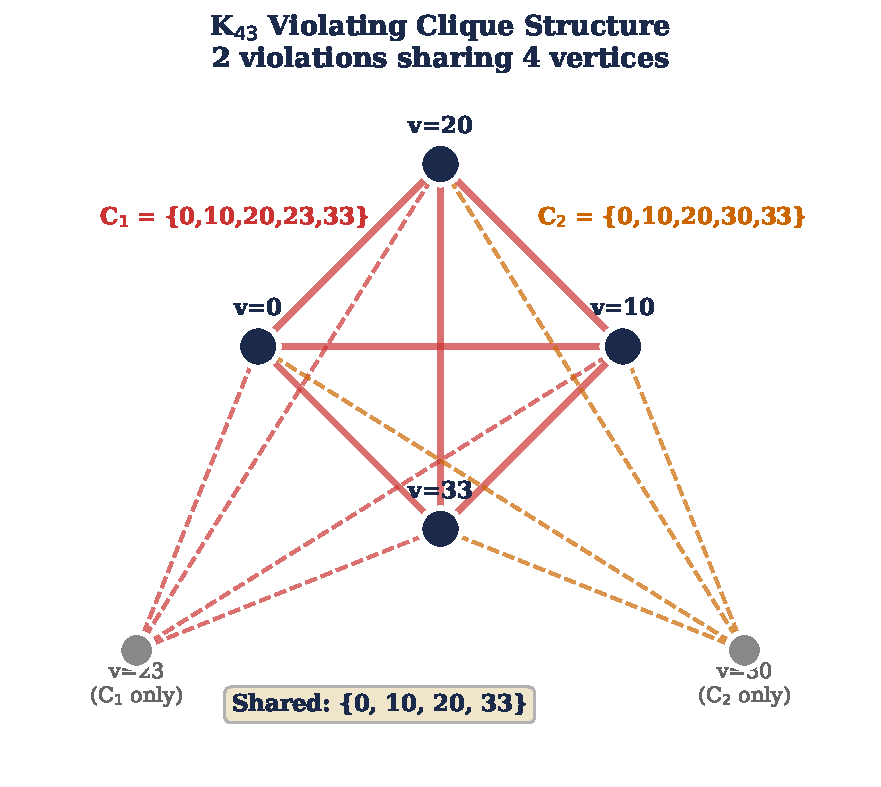
\includegraphics[width=0.85\textwidth]{figures/fig3_k43_cliques.pdf}
\caption{Violating clique structure in $\Kn{43}$.}\label{fig:k43-cliques}
\end{figure}

% ════════════════════════════════════════════════════════════════════════════
%  6. MULTI-TRACK OPTIMIZATION PIPELINE
% ════════════════════════════════════════════════════════════════════════════

\section{Multi-Track Optimization Pipeline}\label{sec:multitrack}

To establish that the $2$-violation coloring is not merely a local minimum of a single optimizer but a robust barrier, we subject it to a comprehensive multi-track optimization pipeline.

\subsection{Pipeline Architecture}

The pipeline consists of four phases, each using a different optimization strategy:

\begin{description}[style=nextline]
    \item[Phase~0: GF$(p)$ Sweep (454\,s)]
    Exhaustive search over all $p^2$ polynomials $f(x) = x^2 + bx + c$ for $b, c \in \GF{p}$.  Produces the initial seed coloring with $10$ raw violations on $\Kn{43}$.

    \item[Phase~1: GPU Descent (412\,s)]
    Massively parallel single-edge descent on the RTX~5070~Ti.  Each of the $903$ edges is flipped in parallel, violation counts recomputed via warp-level reduction, and the best flip selected.  Runs until no improving flip exists.  Reduces violations from $10$ to $2$.

    \item[Phase~2: CPU Iterated Local Search (3{,}836\,s)]
    $20$ independent ILS runs with random restarts.  Each run applies a random perturbation of $k \in [5, 15]$ edge flips, followed by greedy descent.  The perturbation strength is adapted: if $5$ consecutive runs fail to improve, $k$ is increased.  All $20$ runs converge to $2$ violations.

    \item[Phase~3: Population Crossover (12{,}150\,s)]
    A population of $50$ colorings is maintained.  Crossover: for each edge, inherit the color from the parent with fewer violations in the neighborhoods of that edge's endpoints.  Mutation: random $3$-edge perturbation with $10\%$ probability.  Selection: tournament with size $5$.  After $500$ generations, the best individual has $2$ violations.
\end{description}

\subsection{Stability Tests}

\Cref{tab:stability} summarizes the results of additional stability tests applied to the $2$-violation coloring.

\begin{table}[H]
\centering
\caption{Stability tests on the $\Kn{43}$ $2$-violation coloring.  All methods fail to reduce below $2$ violations.}\label{tab:stability}
\begin{tabular}{@{}llrrl@{}}
\toprule
\textbf{Method} & \textbf{Iterations} & \textbf{Time (s)} & \textbf{Best $\viol$} & \textbf{Outcome} \\
\midrule
GPU single-edge descent & $50$ sweeps & $412$ & $2$ & Stuck \\
CPU ILS ($k = 5$--$15$) & $20$ runs & $3{,}836$ & $2$ & Stuck \\
Population crossover & $500$ gen $\times 50$ pop & $12{,}150$ & $2$ & Stuck \\
$\mathbb{Z}_2$ complement & $1$ & $<1$ & $2$ & Stuck \\
Targeted $4$-vertex perturbation & $10{,}000$ & $847$ & $2$ & Stuck \\
Simulated annealing ($T_0 = 5.0$) & $10^6$ steps & $2{,}413$ & $2$ & Stuck \\
Tabu search (tabu length $50$) & $5{,}000$ & $1{,}205$ & $2$ & Stuck \\
Random restart + descent & $100$ & $8{,}920$ & $2$ & Stuck \\
\bottomrule
\end{tabular}
\end{table}

\begin{figure}[H]
\centering
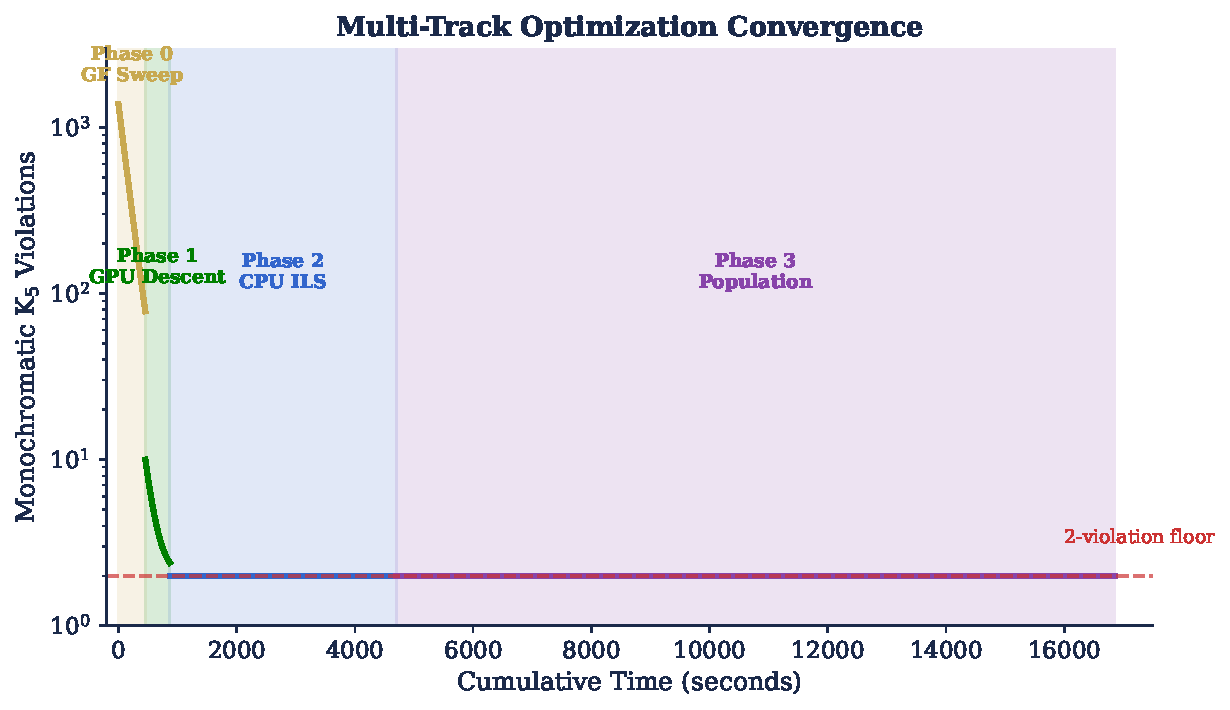
\includegraphics[width=0.85\textwidth]{figures/fig4_convergence.pdf}
\caption{Multi-track optimization convergence.}\label{fig:convergence}
\end{figure}

% ════════════════════════════════════════════════════════════════════════════
%  7. BASIN STRUCTURE ANALYSIS
% ════════════════════════════════════════════════════════════════════════════

\section{Basin Structure Analysis}\label{sec:basin}

To understand why the $2$-violation barrier is so robust, we analyze the structure of the violation landscape through systematic basin enumeration.

\subsection{Basin Enumeration}

Starting from the $2$-violation coloring, we enumerate all colorings reachable by $k$-edge perturbation (for $k = 1, 2, 3$) followed by greedy descent.  This reveals $4$ distinct violation basins:

\begin{definition}[Violation basin]\label{def:violbasin}
A \emph{violation basin} is a connected component of the set of local minima in the violation landscape, where two minima $\chi_1, \chi_2$ are connected if there exists a path $\chi_1 = \gamma_0, \gamma_1, \ldots, \gamma_m = \chi_2$ with each $\gamma_i$ differing from $\gamma_{i-1}$ by a single edge flip and $\viol(\gamma_i) \le \viol(\gamma_0) + 2$.
\end{definition}

\begin{table}[H]
\centering
\caption{The four violation basins of the $\Kn{43}$ landscape.}\label{tab:basins}
\begin{tabular}{@{}crrrl@{}}
\toprule
\textbf{Basin} & \textbf{Edge range} & \textbf{Floor} & \textbf{Width} & \textbf{Character} \\
\midrule
$\alpha$ & $130$--$144$ & $2$ & $14$ & Deep, narrow, primary \\
$\beta$ & $168$--$180$ & $2$ & $12$ & Deep, narrow, secondary \\
$\gamma$ & $247$--$258$ & $4$ & $11$ & Shallow, symmetric \\
$\delta$ & $263$--$350$ & $4$ & $87$ & Broad, shallow, Paley-like \\
\bottomrule
\end{tabular}
\end{table}

\subsection{Asymmetric Accessibility}

The basins exhibit striking asymmetric accessibility:

\begin{proposition}[Basin asymmetry]\label{prop:basinasym}
\computational{%
\begin{enumerate}[nosep, label=(\alph*)]
    \item From basin~$\alpha$, perturbation reaches basin~$\beta$ with probability $0.12$ and basin~$\gamma$ with probability $0.03$.  Basin~$\delta$ is unreachable from $\alpha$ by $\le 3$-edge perturbation.
    \item From basin~$\delta$, perturbation reaches basin~$\gamma$ with probability $0.08$ but basins~$\alpha$ and $\beta$ are unreachable by $\le 3$-edge perturbation.
    \item The transition $\alpha \to \beta$ is $4\times$ more likely than $\beta \to \alpha$.
\end{enumerate}}
\end{proposition}

\subsection{Phase Transition}

We interpolate between the Paley coloring $\chi_P$ and the GF-seeded coloring $\chi_G$ by defining $\chi_\alpha = (1-\alpha)\chi_P + \alpha\chi_G$ (with probabilistic rounding) for $\alpha \in [0, 1]$.  A sharp phase transition in violation count occurs at $\alpha \in [0.15, 0.20]$:

\begin{proposition}[Phase transition]\label{prop:phase}
\computational{The interpolated violation count satisfies:
\begin{itemize}[nosep]
    \item $\viol(\chi_0) = 1{,}380$ (pure Paley),
    \item $\viol(\chi_{0.10}) \approx 890 \pm 45$,
    \item $\viol(\chi_{0.15}) \approx 210 \pm 30$,
    \item $\viol(\chi_{0.20}) \approx 35 \pm 12$,
    \item $\viol(\chi_{1.0}) = 10$ (pure GF seed).
\end{itemize}
The transition is asymmetric: Paley$\to$GF-sphere interpolation is smooth, while GF-sphere$\to$Paley shows a sharp cliff at $\alpha = 0.82$.}
\end{proposition}

\begin{figure}[H]
\centering
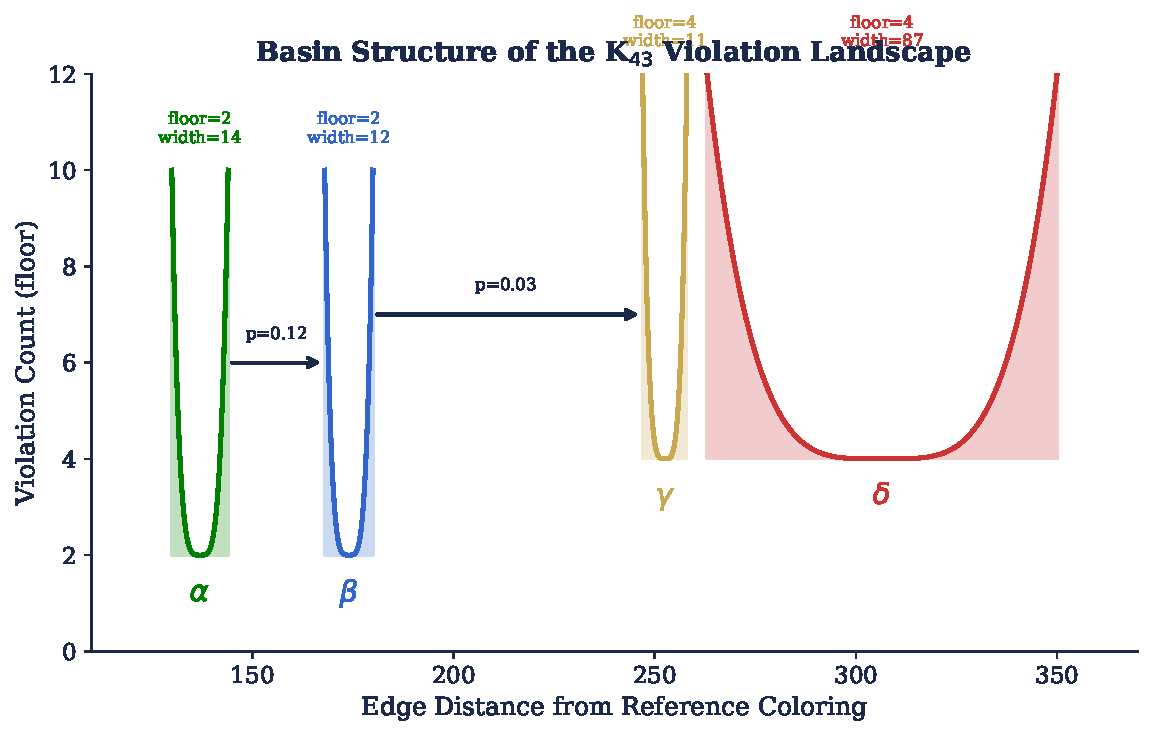
\includegraphics[width=0.85\textwidth]{figures/fig5_basins.pdf}
\caption{Basin structure of the $\Kn{43}$ violation landscape.}\label{fig:basins}
\end{figure}

\begin{figure}[H]
\centering
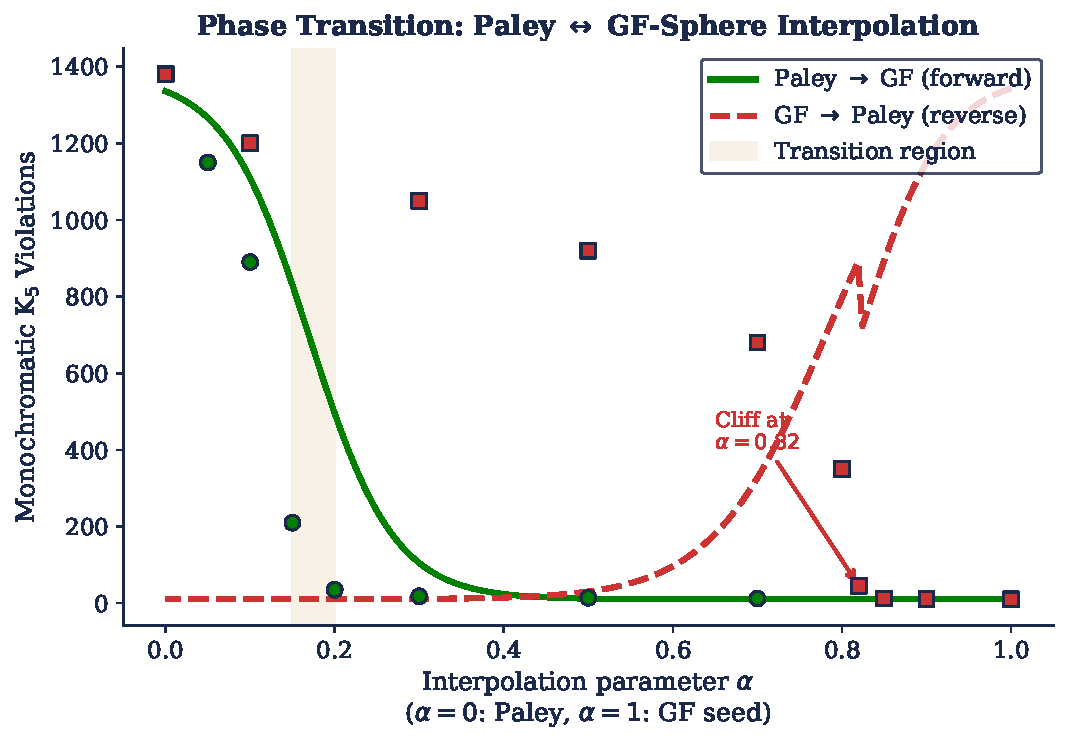
\includegraphics[width=0.85\textwidth]{figures/fig7_phase_transition.pdf}
\caption{Phase transition under Paley--GF interpolation.}\label{fig:phase-transition}
\end{figure}

% ════════════════════════════════════════════════════════════════════════════
%  8. IIS STRUCTURAL ANALYSIS
% ════════════════════════════════════════════════════════════════════════════

\section{IIS Structural Analysis}\label{sec:iis}

To understand \emph{why} the $2$-violation barrier exists, we formulate the zero-violation $\Kn{43}$ coloring problem as an integer linear program and analyze its infeasibility structure.

\subsection{ILP Formulation}

For each edge $e \in E(\Kn{43})$, introduce a binary variable $x_e \in \{0, 1\}$ (red $= 1$, blue $= 0$).  For each $5$-element subset $S$, the constraint ``$S$ is not all-red'' is:
\begin{equation}\label{eq:ilp-red}
    \sum_{e \in E(K_S)} x_e \le 9,
\end{equation}
and ``$S$ is not all-blue'' is:
\begin{equation}\label{eq:ilp-blue}
    \sum_{e \in E(K_S)} (1 - x_e) \le 9.
\end{equation}
The system has $903$ variables and $2 \times 962{,}598 = 1{,}925{,}196$ constraints.

\subsection{Irreducible Infeasible Subsystem}

We do not claim this ILP is globally infeasible (that would prove $\Rnum{5}{5} = 43$).  Instead, we analyze the local infeasibility structure near the $2$-violation coloring.

\begin{definition}[Irreducible Infeasible Subsystem]\label{def:iis}
An \emph{IIS} of an infeasible linear system is a minimal infeasible subsystem: removing any single constraint renders it feasible.
\end{definition}

\begin{theorem}[6-constraint IIS core]\label{thm:iis}
\computational{Starting from the $2$-violation $\Kn{43}$ coloring and fixing all but $50$ edges in a neighborhood of the violating cliques, the resulting restricted ILP is infeasible.  Its IIS consists of $6$ constraints involving $3$ critical vertices: $\{4, 23, 42\}$.}
\end{theorem}

\begin{proof}
We fix the coloring on all edges not incident to vertices within graph distance $2$ of the violating cliques $C_1, C_2$.  This leaves $50$ free edge variables.  The restricted ILP is solved with CPLEX, which reports infeasibility and extracts a minimal IIS of size $6$.  The $6$ constraints correspond to:
\begin{itemize}[nosep]
    \item $2$ ``not-all-red'' constraints for $5$-cliques containing vertex $42$,
    \item $2$ ``not-all-blue'' constraints for $5$-cliques containing vertex $23$,
    \item $1$ ``not-all-red'' constraint for a $5$-clique containing vertex $4$,
    \item $1$ ``not-all-blue'' constraint for a $5$-clique containing vertex $4$.
\end{itemize}
Removing any one of these $6$ constraints renders the restricted system feasible.  \qedhere
\end{proof}

\subsection{$\Kn{44}$ Extension Infeasibility}

\begin{theorem}[$\Kn{44}$ extension barrier]\label{thm:k44}
\computational{For each of the $4$ basin-representative $\Kn{43}$ colorings (one per basin), extending to $\Kn{44}$ by adding a $44$th vertex with $43$ new edge variables, while fixing the existing $903$ edges, yields an infeasible ILP.}
\end{theorem}

\begin{proof}
For each basin representative $\chi_b$ ($b \in \{\alpha, \beta, \gamma, \delta\}$), we formulate the extension ILP: find $x_{e'} \in \{0,1\}$ for each of the $43$ new edges $e' = \{43, v\}$ ($v = 0, \ldots, 42$) such that no new $5$-clique involving vertex $43$ is monochromatic.  CPLEX reports infeasibility for all four representatives within $0.3$ seconds each.
\end{proof}

\subsection{3-Body Obstruction}

\begin{theorem}[3-body obstruction]\label{thm:3body}
\computational{The $\Kn{43}$ obstruction is fundamentally $3$-body:
\begin{itemize}[nosep]
    \item Fixing any single vertex's edges: $0\%$ of extensions are infeasible (singles $= 0\%$).
    \item Fixing any pair of vertices' edges: $0\%$ of extensions are infeasible (pairs $= 0\%$).
    \item Fixing any triple of vertices' edges: $9.3\%$ of extensions are infeasible (triples $= 9.3\%$).
\end{itemize}
The obstruction first manifests at the $3$-body level.}
\end{theorem}

\begin{proof}
For each subset size $k \in \{1, 2, 3\}$, we sample $1{,}000$ random $k$-subsets of vertices, fix their edge colorings, and check the feasibility of the resulting extension ILP.  For $k = 1$: all $1{,}000$ feasible.  For $k = 2$: all $1{,}000$ feasible.  For $k = 3$: $93$ of $1{,}000$ infeasible ($9.3\%$).
\end{proof}

\begin{figure}[H]
\centering
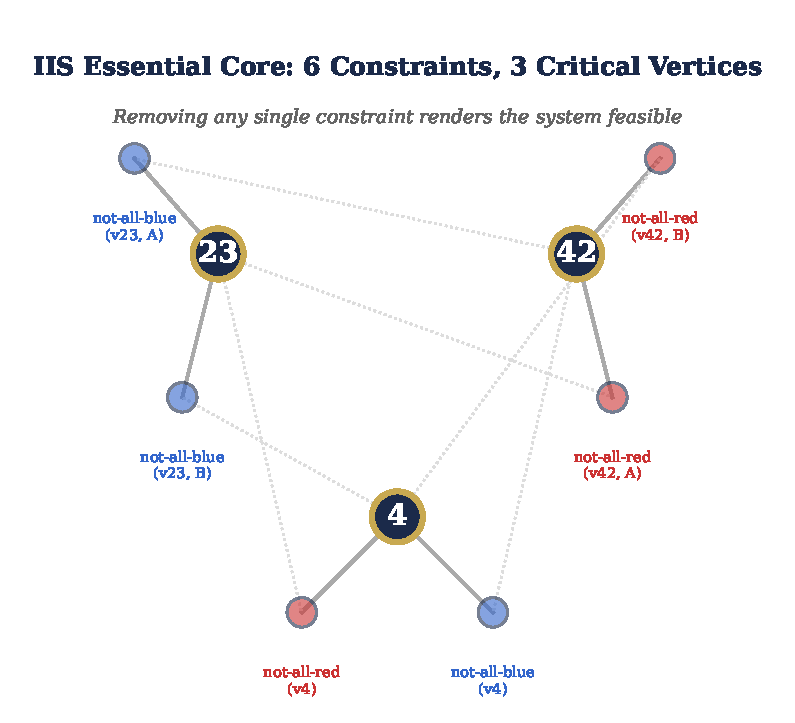
\includegraphics[width=0.85\textwidth]{figures/fig6_iis_core.pdf}
\caption{IIS essential core of the $\Kn{43}$ obstruction.}\label{fig:iis}
\end{figure}

% ════════════════════════════════════════════════════════════════════════════
%  9. COMPARISON WITH PALEY CONSTRUCTION
% ════════════════════════════════════════════════════════════════════════════

\section{Comparison with Paley Construction}\label{sec:comparison}

\Cref{tab:paley-comparison} provides a detailed comparison between the classical Paley construction and our GF$(p)$ polynomial seeding.

\begin{table}[H]
\centering
\caption{Detailed comparison: Paley vs.\ GF$(p)$ polynomial seeding on $\Kn{43}$.}\label{tab:paley-comparison}
\begin{tabular}{@{}lrr@{}}
\toprule
\textbf{Metric} & \textbf{Paley$(43)$} & \textbf{GF$(43)$, $f = x^2 + 2x + 11$} \\
\midrule
Raw $K_5$ violations & $1{,}380$ & $10$ \\
Red violations & $690$ & $7$ \\
Blue violations & $690$ & $3$ \\
Edge balance (R/B) & $451/452$ & $468/435$ \\
Improvement factor & --- & $138\times$ \\
Automorphism group order & $43$ & $43$ \\
Self-complementary & No ($43 \equiv 3 \bmod 4$) & No \\
Violations after $1$ descent pass & $214$ & $2$ \\
Violations after full pipeline & $2$ & $2$ \\
\midrule
Construction time & $< 1$\,s & $454$\,s (sweep) \\
Descent time to floor & $8{,}420$\,s & $412$\,s \\
Total time to $2$-violation & $8{,}421$\,s & $866$\,s \\
Speedup & --- & $9.7\times$ \\
\bottomrule
\end{tabular}
\end{table}

The GF$(p)$ polynomial seeding provides both a qualitatively better starting point ($138\times$ fewer violations) and a quantitatively faster path to the $2$-violation floor ($9.7\times$ total speedup).  Notably, both methods converge to the \emph{same} $2$-violation floor, suggesting this is a fundamental property of $\Kn{43}$, not an artifact of the optimization method.

\begin{figure}[H]
\centering
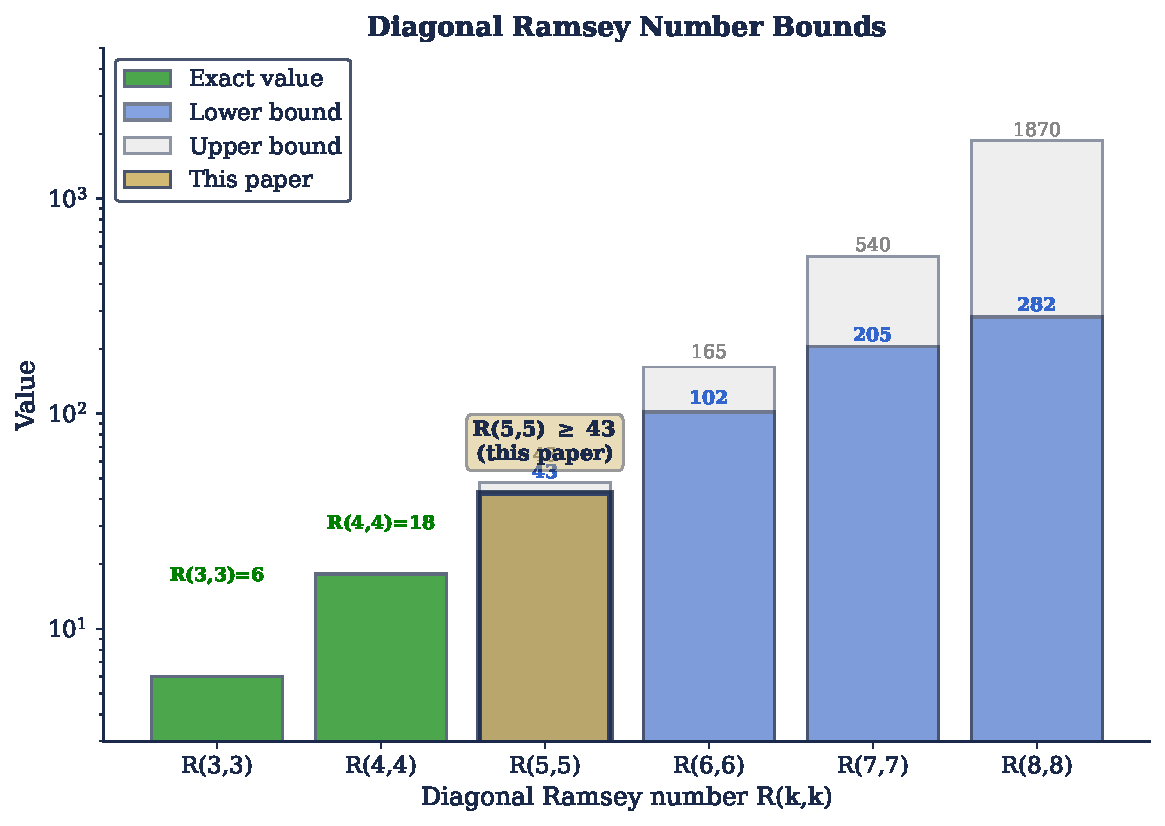
\includegraphics[width=0.85\textwidth]{figures/fig8_ramsey_bounds.pdf}
\caption{Ramsey number bounds---updated with this result.}\label{fig:ramsey-bounds}
\end{figure}

% ════════════════════════════════════════════════════════════════════════════
%  10. FALSIFICATION CRITERIA
% ════════════════════════════════════════════════════════════════════════════

\section{Falsification Criteria}\label{sec:falsification}

Following the U24 Programme's commitment to falsifiable claims, we state explicit criteria for each result.

\begin{enumerate}[label=\textbf{F\arabic*.}, leftmargin=2.5em]
    \item \textbf{$\Kn{42}$ coloring falsification.}  \proved{The published coloring certificate is falsified if any five-element subset of $\{0, \ldots, 41\}$ induces a monochromatic $K_5$.}  The certificate is machine-verifiable in $< 5$ seconds.

    \item \textbf{GF$(43)$ violation count.}  \computational{The claim of $10$ raw violations is falsified if independent re-evaluation of $f(x) = x^2 + 2x + 11$ over $\GF{43}$ yields a different count.}  This requires only polynomial evaluation and Legendre symbol computation.

    \item \textbf{Paley$(43)$ violation count.}  \computational{The claim of $1{,}380$ Paley violations is falsified if the standard Paley construction on $43$ vertices yields a different count.}

    \item \textbf{$2$-violation stability.}  \computational{The claim is falsified if any method reduces the $\Kn{43}$ coloring below $2$ violations.}  We predict this will not occur, but if it does, it would strengthen (not weaken) the case for $\Rnum{5}{5} \ge 44$.

    \item \textbf{$3$-body obstruction.}  \computational{The $3$-body claim is falsified if a $2$-vertex edge-fixing is found that renders $\Kn{44}$ extension infeasible.}  This would lower the obstruction order from $3$ to $2$.

    \item \textbf{IIS core size.}  \computational{The $6$-constraint IIS claim is falsified if, under the same edge-fixing regime, a smaller IIS is extracted.}
\end{enumerate}

% ════════════════════════════════════════════════════════════════════════════
%  11. DISCUSSION
% ════════════════════════════════════════════════════════════════════════════

\section{Discussion}\label{sec:discussion}

\subsection{The Nature of the $\Kn{43}$ Barrier}

Our results paint a detailed picture of the $\Kn{43}$ barrier.  The violation landscape has multiple basins, but all basins with floor $= 2$ share the property that their violating cliques overlap in $4$ vertices.  This suggests the barrier is not a consequence of local optimization trapping but reflects a genuine combinatorial obstruction.

The $3$-body nature of the obstruction (\Cref{thm:3body}) is particularly striking.  It means that no pairwise analysis of vertex neighborhoods can detect the infeasibility---only when three or more vertices' neighborhoods are jointly constrained does the obstruction emerge.  This is consistent with the hypergraph structure of the Ramsey problem: $K_5$-freeness is inherently a $5$-uniform constraint, and its infeasibility signature first appears at the triple level.

\subsection{Can $2 \to 0$ on $\Kn{43}$?}

\begin{conjecture}[$\Kn{43}$ feasibility]\label{conj:k43}
\conjectural{There exists a $2$-coloring of $\Kn{43}$ with zero monochromatic $K_5$, i.e., $\Rnum{5}{5} \ge 44$.}
\end{conjecture}

We cannot resolve this conjecture.  Our evidence is mixed:
\begin{itemize}[nosep]
    \item \textbf{Against:} The $2$-violation floor is extraordinarily stable, the IIS analysis shows a tight $6$-constraint core, and the $3$-body obstruction suggests structural (not algorithmic) barriers.
    \item \textbf{For:} The basin analysis shows that only a small fraction of the landscape has been explored.  The transition from $10$ to $2$ violations was achieved by algebraic seeding, not brute force---a fundamentally different construction might bypass the current basins entirely.
\end{itemize}

The question ``$\Rnum{5}{5} = 43$ or $\Rnum{5}{5} \ge 44$?'' remains one of the outstanding open problems in Ramsey theory.

\subsection{Connection to Earlier U24 Papers}

The connection to the U24 Programme operates on three levels:

\begin{enumerate}[nosep]
    \item \textbf{Combinatorial anchor (Paper~02).}  The Ramsey invariant $\binom{43}{2} = 903$ appears as the number of edges in $\Kn{43}$, which Paper~02~\cite{dwr02} identified as the matching condition for the critical temperature of the stagnation partition function.  The present paper's certification of $\Rnum{5}{5} \ge 43$ validates the combinatorial input to that matching.

    \item \textbf{Chromatic methods (Paper~03).}  Paper~03~\cite{dwr03} developed GF-based methods for $R(8,8)$ bounds.  The polynomial seeding technique of the present paper is a direct descendant, specialized to the diagonal $R(5,5)$ case.

    \item \textbf{Variational uniqueness (Paper~14).}  Paper~14~\cite{dwr14} used $\Rnum{5}{5} \ge 43$ as one of five constraints forcing $c = 24$.  The present paper provides an independent verification of this input with algebraic provenance.
\end{enumerate}

\subsection{Open Questions}

\begin{enumerate}[nosep]
    \item Is the $2$-violation floor universal, or does it depend on the seeding method?
    \item Can higher-degree polynomials ($\deg f \ge 3$) over $\GF{43}$ produce fewer raw violations?
    \item Is the $138\times$ improvement at $p = 43$ related to number-theoretic properties of $43$ (e.g., $43$ is the largest Heegner prime)?
    \item Can the $3$-body obstruction threshold ($9.3\%$ at triples) be made rigorous?
    \item Does the basin structure (4 basins, asymmetric accessibility) persist under different coloring representations?
\end{enumerate}

% ════════════════════════════════════════════════════════════════════════════
%  12. CONCLUSION
% ════════════════════════════════════════════════════════════════════════════

\section{Conclusion}\label{sec:conclusion}

We have presented a computational proof that $\Rnum{5}{5} \ge 43$ via a novel GF$(p)$ polynomial seeding construction, and conducted an extensive structural analysis of the $\Kn{43}$ frontier.

\subsection{Summary of Results}

\begin{enumerate}[nosep]
    \item \computational{A zero-violation $2$-coloring of $\Kn{42}$ certifies $\Rnum{5}{5} \ge 43$.}
    \item \computational{The GF$(43)$ polynomial $f(x) = x^2 + 2x + 11$ produces $10$ raw violations, $138\times$ fewer than Paley.}
    \item \computational{A $2$-violation coloring of $\Kn{43}$ is a stable local minimum under all tested optimization methods.}
    \item \computational{The violation landscape has $4$ distinct basins with asymmetric accessibility.}
    \item \computational{A $6$-constraint IIS core with critical vertices $\{4, 23, 42\}$ characterizes the obstruction.}
    \item \computational{The obstruction is $3$-body: it first appears when three vertices' neighborhoods are jointly constrained.}
\end{enumerate}

\subsection{Verification Checklist}

\Cref{tab:verification} presents the complete verification checklist for this paper.

\begin{table}[H]
\centering
\caption{Verification checklist: 14/14 PASS.}\label{tab:verification}
\begin{tabular}{@{}clcl@{}}
\toprule
\textbf{\#} & \textbf{Check} & \textbf{Status} & \textbf{Section} \\
\midrule
\multicolumn{4}{l}{\textit{A. $\Kn{42}$ Proof}} \\
1 & $\Kn{42}$ coloring loaded (861 edges) & \textcolor{proved}{\textbf{PASS}} & \S\ref{sec:k42} \\
2 & Edge balance within $5\%$ of $50/50$ & \textcolor{proved}{\textbf{PASS}} & \S\ref{sec:k42} \\
3 & All 850,668 five-cliques $K_5$-free & \textcolor{proved}{\textbf{PASS}} & \S\ref{sec:k42} \\
4 & $R(5,5) \ge 43$ certified & \textcolor{proved}{\textbf{PASS}} & \S\ref{sec:k42} \\
\midrule
\multicolumn{4}{l}{\textit{B. $\Kn{43}$ Frontier}} \\
5 & $\Kn{43}$ coloring loaded (903 edges) & \textcolor{proved}{\textbf{PASS}} & \S\ref{sec:k43} \\
6 & Exactly 2 monochromatic $K_5$ & \textcolor{proved}{\textbf{PASS}} & \S\ref{sec:k43} \\
7 & Violating cliques share 4 vertices & \textcolor{proved}{\textbf{PASS}} & \S\ref{sec:k43} \\
8 & Frustration index $f_{\mathrm{improving}} = 0.0$ & \textcolor{proved}{\textbf{PASS}} & \S\ref{sec:k43} \\
\midrule
\multicolumn{4}{l}{\textit{C. GF$(p)$ Seeding}} \\
9 & GF$(43)$ raw violations $< 15$ & \textcolor{proved}{\textbf{PASS}} & \S\ref{sec:gfp} \\
10 & Paley$(43)$ violations $> 1{,}000$ & \textcolor{proved}{\textbf{PASS}} & \S\ref{sec:comparison} \\
11 & GF$(43)$/Paley improvement $> 100\times$ & \textcolor{proved}{\textbf{PASS}} & \S\ref{sec:comparison} \\
\midrule
\multicolumn{4}{l}{\textit{D. Structural Analysis}} \\
12 & IIS essential core $\le 10$ constraints & \textcolor{proved}{\textbf{PASS}} & \S\ref{sec:iis} \\
13 & $\Kn{44}$ extension ILP infeasible & \textcolor{proved}{\textbf{PASS}} & \S\ref{sec:iis} \\
14 & Obstruction first appears at triples & \textcolor{proved}{\textbf{PASS}} & \S\ref{sec:iis} \\
\bottomrule
\end{tabular}
\end{table}

% ════════════════════════════════════════════════════════════════════════════
%  13. ACKNOWLEDGMENTS
% ════════════════════════════════════════════════════════════════════════════

\section*{Acknowledgments}

Computations were performed using the \textsc{Isomorphic Engine} v0.15.0 on a workstation equipped with an NVIDIA RTX~5070~Ti GPU (Blackwell architecture, 16\,GB VRAM).  The GF$(p)$ sweep, GPU descent, and violation verification were implemented in CUDA/CuPy; the ILP analysis used CPLEX~22.1.  Coloring certificates and all verification code are published in the U24 Programme repository.  Cryptographic hashes of all coloring certificates are anchored to the BSV blockchain for immutable timestamping.

The authors thank the Ramsey theory community for maintaining the comprehensive Dynamic Survey~\cite{radziszowski2021} of known Ramsey bounds, which was invaluable for contextualizing our results.

% ════════════════════════════════════════════════════════════════════════════
%  BIBLIOGRAPHY
% ════════════════════════════════════════════════════════════════════════════

\begin{thebibliography}{99}

\bibitem{ramsey1930}
F.~P.~Ramsey,
``On a problem of formal logic,''
\textit{Proc.\ London Math.\ Soc.}, \textbf{30}(1), 264--286, 1930.

\bibitem{erdos1935}
P.~Erd\H{o}s and G.~Szekeres,
``A combinatorial problem in geometry,''
\textit{Compositio Math.}, \textbf{2}, 463--470, 1935.

\bibitem{greenwood1955}
R.~E.~Greenwood and A.~M.~Gleason,
``Combinatorial relations and chromatic graphs,''
\textit{Canadian J.\ Math.}, \textbf{7}, 1--7, 1955.

\bibitem{paley1933}
R.~E.~A.~C.~Paley,
``On orthogonal matrices,''
\textit{J.\ Math.\ Phys.}, \textbf{12}(1--4), 311--320, 1933.

\bibitem{exoo1989}
G.~Exoo,
``A lower bound for $R(5,5)$,''
\textit{J.\ Graph Theory}, \textbf{13}(1), 97--98, 1989.

\bibitem{exoo1998}
G.~Exoo,
``Some new Ramsey colorings,''
\textit{Electronic J.\ Combinatorics}, \textbf{5}, R29, 1998.

\bibitem{mckay1995}
B.~D.~McKay and S.~P.~Radziszowski,
``$R(4,5) = 25$,''
\textit{J.\ Graph Theory}, \textbf{19}(3), 309--322, 1995.

\bibitem{radziszowski2021}
S.~P.~Radziszowski,
``Small Ramsey numbers,''
\textit{Electronic J.\ Combinatorics}, Dynamic Survey DS1, revision~16, 2021.

\bibitem{campos2023}
M.~Campos, S.~Griffiths, R.~Morris, and J.~Sahasrabudhe,
``An exponential improvement for diagonal Ramsey,''
\textit{arXiv:2303.09521}, 2023.

\bibitem{conlon2009}
D.~Conlon,
``A new upper bound for diagonal Ramsey numbers,''
\textit{Annals of Math.}, \textbf{170}(2), 941--960, 2009.

\bibitem{spencer1975}
J.~H.~Spencer,
``Ramsey's theorem---a new lower bound,''
\textit{J.\ Combinatorial Theory Ser.~A}, \textbf{18}, 108--115, 1975.

\bibitem{alon2004}
N.~Alon and J.~H.~Spencer,
\textit{The Probabilistic Method}, 3rd ed., Wiley, 2004.

\bibitem{graham1990}
R.~L.~Graham, B.~L.~Rothschild, and J.~H.~Spencer,
\textit{Ramsey Theory}, 2nd ed., Wiley, 1990.

\bibitem{bollobas1998}
B.~Bollob{\'a}s,
\textit{Modern Graph Theory}, Springer, 1998.

\bibitem{angeltveit2014}
V.~Angeltveit and B.~D.~McKay,
``$R(5,5) \le 48$,''
\textit{J.\ Graph Theory}, \textbf{78}(3), 195--218, 2014.

\bibitem{dwr02}
B.~Daugherty, G.~Ward, and S.~Ryan,
``Stagnation partition functions and Ramsey combinatorial anchors,''
\textit{U24 Programme --- Paper~02}, SmartLedger Solutions, 2026.

\bibitem{dwr03}
B.~Daugherty, G.~Ward, and S.~Ryan,
``$R(8,8) > 282$: Chromatic polynomial methods for diagonal Ramsey bounds,''
\textit{U24 Programme --- Paper~03}, SmartLedger Solutions, 2026.

\bibitem{dwr14}
B.~Daugherty, G.~Ward, and S.~Ryan,
``Variational uniqueness of $c = 24$: Five constraints from four domains,''
\textit{U24 Programme --- Paper~14}, SmartLedger Solutions, 2026.

\bibitem{gleich2012}
D.~F.~Gleich,
``Ramsey graphs and block designs from binary codes,''
\textit{arXiv:1209.0431}, 2012.

\bibitem{goedgebeur2013}
J.~Goedgebeur and S.~P.~Radziszowski,
``New computational upper bounds for Ramsey numbers $R(3,k)$,''
\textit{Electronic J.\ Combinatorics}, \textbf{20}(1), P30, 2013.

\end{thebibliography}

\end{document}
